\chapter{Control approach}\label{ch:controlapproach3D}


\section{Control strategy}\label{sec:3DcontrolSimplisticStrategy}
\noindent Main purpose of control strategy is to define discrete set of moves which can be later used in approximation models. Therefore vehicle velocity is set to constant speed $v_v = 1\quad m/s$ because increasing and decreasing speed can make predicted trajectories malformed. It is needed to distinguish between \textit{control strategy} $\Omega(t)$ and \textit{control set} $U(t)$. \textit{Control set} $U(t)$ contains all available control inputs regardless vehicle state and surrounding. \textit{Control strategy} $\Omega(t)$ contains only control inputs $\omega(t)$ which keeps vehicle in safe invariant reachable set $\mathscr{R}$.
\begin{equation}\label{simple3dControlSet}
    u(t)\in U(T) =
    \begin{cases}
        \left [ v_c,0,0,0 \right ]^T & :s_0 \quad\textnormal{fly straight} \\
        \left [ v_c,0,\frac{\pi}{12},0 \right ]^T & :s_1 \quad\textnormal{fly downward} \\
        \left [ v_c,0,-\frac{\pi}{12},0 \right ]^T & :s_2 \quad\textnormal{fly upward} \\
        \left [ v_c,0,0,\frac{\pi}{12} \right ]^T & :s_3 \quad\textnormal{fly left} \\
        \left [ v_c,0,0,-\frac{\pi}{12} \right ]^T & :s_4 \quad\textnormal{fly right} 
    \end{cases}
\end{equation}
Control set $U(t)$ (\ref{simple3dControlSet}) contains five basic movement which affects yaw or pitch angular velocity. This allows us to develop movement set containing basic movement like fly straight, fly upward, fly downward, fly left and fly right. Movement set  is designed to cover maximum maneuverability. From viewpoint of reachable control set $U(t)$ have maximal maneuverability subset $\Gamma(t)$ which contains only maneuvers which are on border of reach set. Maximal maneuverability subset $\Gamma(t)$ is equal to control set $U(t)$ in this case. For example les sharp turn to right $u(t)=\left [ v_c,0,0,-\frac{\pi}{16} \right ]^T$ will be member of control set $U(t)$, but will not be member of maximal maneuverability set $\Gamma(t)$, because there exist sharper turn to right $u(t) = \left [ v_c,0,0,-\frac{\pi}{12} \right ]^T $. Maximal maneuverability set $\Gamma(t)$ is used in estimation of invariant safe reach set $\mathscr{R}$.

\newpage
\section{Path finding in partially known environment}
\noindent Path finding in partially known environment is nontrivial task which requires additional safety margin. Firstly visibility field $\mathscr{F}_{3D}$ needs to be defined for single time snapshot, then it can be extended to trajectory.
\subsection{Visibility field}
\begin{definition}{Visibility field in third dimension $\mathscr{F}_{3D}$}\label{def:VisibleSpace}
    Let $x_0=[0,0,0]^T$ be observation point and X axis as directional axis, horizontal view limiter on XY plane as $[\theta_S,\theta_E]$, vertical view limiter on XZ plane as $[\varphi_S,\varphi_E]$ and view distance as $d_v$.
    \\
    Then point $x_p=[x,y,z]\in R^3$ with horizontal angle $\theta_p = \arctan y/x$, vertical angle $\varphi_p=\arctan z/x$  and $d_p=\norm{x_p}$ belongs to visibility field if and only if:
    \begin{equation}
        0 \le d_p \le d_v
    \end{equation}
    \begin{equation}
        \theta_S \le \theta_p \le \theta_E
    \end{equation}
    \begin{equation}
        \varphi_S \le \varphi_p \le \varphi_E
    \end{equation}
\end{definition}
\noindent\textit{Visibility field} $\mathscr{F}_{3D}$ can be divined into \textit{visibility grid} $\mathscr{G}_{3D}$ to ease computational complexity, this approach is taken from \cite{goerzen2010survey}. This approach is based on fast classification of obstacle space $\mathscr{O}_{3D}$ and uncertain space $\mathscr{U}_{3D}$ in field of vision $\mathscr{F}_{3D}$. Cell size can be scaled to needs of path finding algorithm.
\begin{definition}{Visibility grid cell $c_{i,j,k}\in\N^+$}\label{def:visibilityGridCell}
    in grid is with defined position by layer index $k\in\{1\dots l_c\}$, column index $j\in\{1\dots h_c\}$ and  row index $i\in\{1\dots v_c\}$, where $l_c\in\N^+$ is layer count, $v_c\in\N^+$ is vertical cell count, $h_c\in\N^+$ is horizontal cell count. Example of grid cell can be found in figure \ref{fig:62VisibilityGridCellExample}.
    \begin{figure}[H]
        \centering
        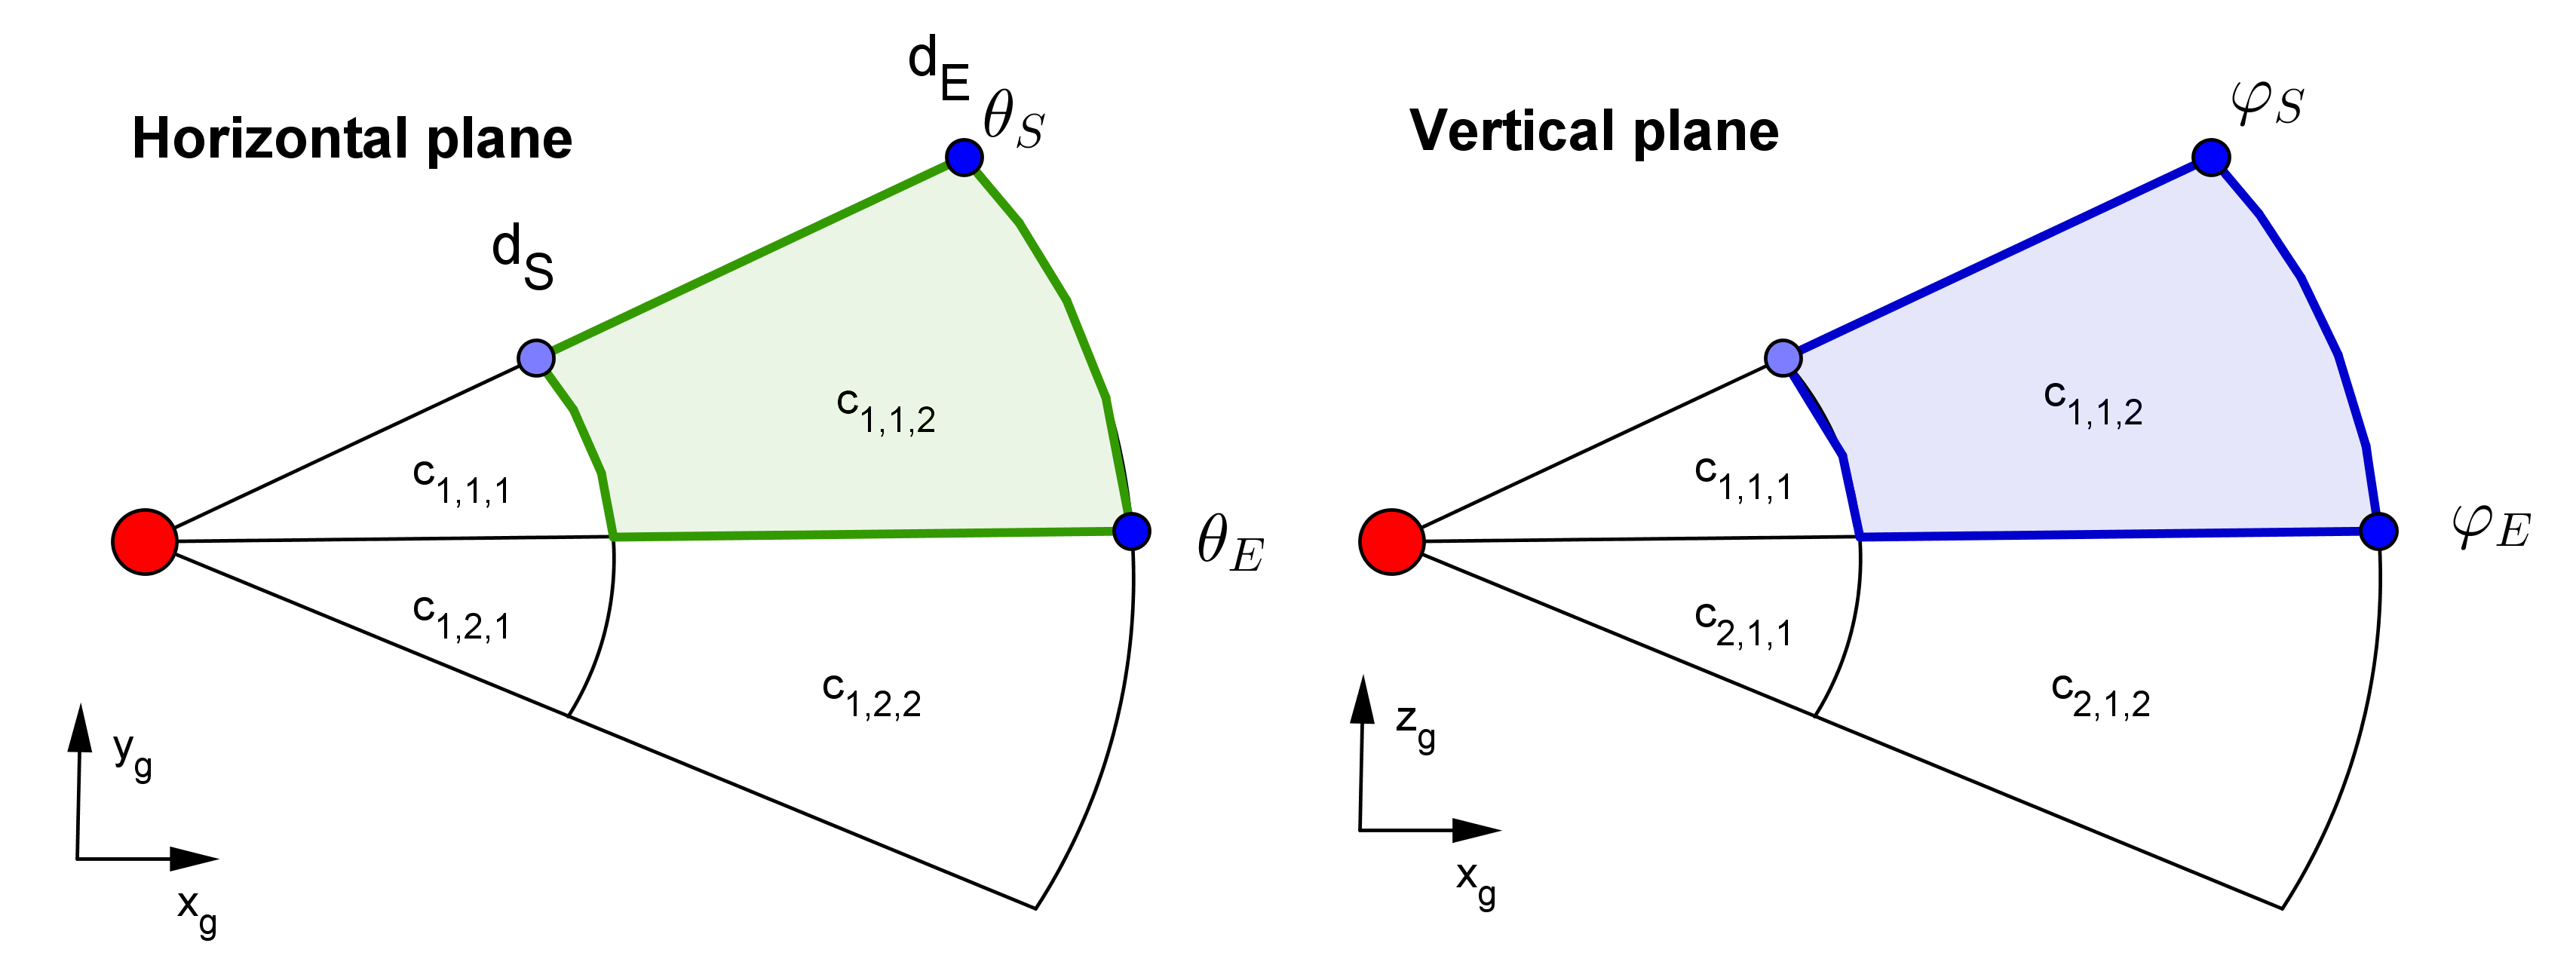
\includegraphics[width=0.8\linewidth]{\FIGDIR/62_Visibility_Grid_Cell_example.png}
        \caption{Visibility grid cell $c_{1,1,2}$ example.}
        \label{fig:62VisibilityGridCellExample}
    \end{figure}
    Visibility grid cell occupied space is defined by $[d_s,d_e,\theta_s,\theta_e,\varphi_s,\varphi_e]$, where $(d_s,d_e]\in\R^2$ distance range, $(\theta_s,\theta_r$ is horizontal range and $(\varphi_s,\varphi_e]$ is vertical range. Then point $x_p=[x,y,z]\in R^3$ with horizontal angle $\theta_p = \arctan y/x$, vertical angle $\varphi_p=\arctan z/x$  and $d_p=\norm{x_p}$ belongs to visibility grid cell $c_{i,j,k}\in\N^+$ if and only if:
    \begin{equation}
        d_s \le d_p \le d_e
    \end{equation}
    \begin{equation}
        \theta_s \le \theta_p \le \theta_e
    \end{equation}
    \begin{equation}
        \varphi_s \le \varphi_p \le \varphi_e
    \end{equation}
    \newpage\noindent    
    Visibility grid cell have defined state property s:
    \begin{enumerate}
        \item \textit{Not determined} - state of cell have not been determined, because it does not complain with any following status rule.
        \item \textit{Reachable} - cell is reachable and there exist control input $u(t)$ which will bring position state $[x_p(t),y_p(t),z_p(t)]^T$ to any point belonging to cell from grid origin $[0,0,0]^T$, and any point of trajectory $[x_p(t),y_p(t),z_p(t)]^T$ does not belong to grid cell with Obstacle or Uncertain state.
        \item \textit{Unreachable} - cell is unreachable and there does not exist any control input $u(t)$ which comply with reachibility rule.
        \item \textit{Obstacle} - cell contains at least one detected obstacle point from obstacle set $\mathscr{O}_{3D}$.
        \item \textit{Uncertain} - cell visibility is hindered by obstacle cell or uncertain cell on previous layer.
        \item \textit{Goal} - cell center is closest to goal waypoint $\mathscr{WP}_{goal}$.
    \end{enumerate}
    \textit{Successors} is set of cells directly or partially covered in line of sight by selected cell $c_{i,j,k}$. \textit{Predecessors} is set of cells directly or partially covering line of sight of selected cell $c_{i,j,k}$.
\end{definition}
\noindent For  further definition of partially known environment definitions of  visibility grid (\ref{def:VisibleSpace}), visibility grid cell (\ref{def:visibilityGridCell}), local obstacle position transformation (\ref{def:globalObstaclePosition3D}). Let say that system $\dot{x} = f(x,u)$ finishes scanning of surrounding environment at time $t_i$ in visibility grid defined by  parameters $[d,\theta_S,\theta_E,\varphi_S,\varphi_E,l_c,h_c,v_c]$. Then $\mathscr{F}_{3d}(t_i)$ gives situation valid for small time frame $[t_i,t_{i+1})$, where $t_{i+1}$ is time of new full surrounding environment scan. 

In this operational frame three distances are setup $0 \le d_p \le d_o \le  d_u \le d$ where $d_p$ is processing distance, $d_o$ is operational distance and $d_u$ is unsafe distance. Processing distance $d_p$ is is maximal distance in which avoidance maneuvers are processed. Operational distance $d_o$ is distance in which  any avoidance maneuver is safe. Unsafe distance $d_u$ is a distance in which avoidance maneuver may lead to crash. Example of avoidance frame overlapping can be found in figure \ref{fig:visibleVsReachableLocalFrame}. Following assumptions have been taken into account:

\begin{assumption}{Processing distance $d_p$ is equal to 0, therefore result of avoidance engine is known at time of detection $t_i$.}\label{ass:7}\end{assumption}
\begin{assumption}{Unsafe distance $d_u$ is equal to visibility distance $d$.}\label{ass:8}\end{assumption}
\noindent For better imagination what this assumptions have done on presented avoidance principle is summarized in following outcome of assumptions \ref{ass:7}. and \ref{ass:8}:
\begin{enumerate}
    \item Avoidance area $\mathscr{A}(t_i)$ is equal to visibility field $\mathscr{F}_{3D}(t_i)$.
    \item There is no unsafe area because $d_u=d$.
    \item Controlable origin (point where you can change vehicle trajectory) is at origin of $\mathscr{F}_{3D}$.
\end{enumerate}

\subsection{Pre-calculated reach set approach}
\noindent To minimize computation time of reachable space for system $\dot{x}=f(x,u)$, with movement automaton $\mathscr{MA}$ given by definition \ref{def:movementAutomaton} in Visibility grid $\mathscr{G}_{3D}$ given by definition \ref{def:VisibleSpace} partitioned into visibility cells $c_{i,j,k}\in \mathscr{G}_{3D}$ given by definition \ref{def:visibilityGridCell} two stage computation method is presented. 
\begin{enumerate}
    \item \textit{First stage} is to create numeric approximation of Reach set in $\mathscr{G}_{3D}$ where all visibility grid cells are considered as \textit{Not determined} state.
    \item \textit{Second stage} is to use pre-calculated structure and prune it with \textit{Obstacles} and \textit{Uncertain} cells popping in.
\end{enumerate}
 This approach allows us to use heavy computational methods in first stage and removing bias of additional calculations from second stage. Second stage is used every obstacle avoidance framework run. First stage is used only in case of following events:
\begin{enumerate}
    \item \textit{System equation change} - when system $\dot{x}=f(x,u)$ changes, this can be invoked by payload or weather condition change, prior the mission execution.
    \item \textit{Control strategy change} - when control strategy $u(t)\in U(t)$ changes, this can be invoked by control constraints change.
    \item \textit{Movement set change} - movement automaton $\mathscr{MA}$ has finite set of movements $m_i\in M$, when this set changes reach set estimation structure needs to be recalculated due the estimation method dependence. 
\end{enumerate}

\noindent\textit{Trajectory representation} is key in this approximation method. Reach set $\mathscr{R}[t_0,t_1,x_0]$ can be represented as set of all trajectories reachable from starting point $x_0$ at time $t_0$ up to end time $t_1$. Reduction of reach set from closed compact set $\mathscr{R}\subset \R^N$ to closed compact set of movement chains $\mathscr{R}\subset M^m, m\in\N^+$ is granted trough using movement automaton $\mathscr{MA}$ as control input in closed control loop for system $\dot{x} = f(x,u)$.

\begin{definition}{Trajectory $\mathscr{T}(x_0,B)$.}\label{def:movementTrajectory} 
    System given by equation $\dot{x}=f(x,u)$ with state vector $x\in \R^n$ and input vector $u \in \R^M$, where control input is $u(t)$ is generated by movement automaton $\mathscr{MA}$. Set of available movements is given by $M\in\mathscr{MA}$, where buffer $B$ ordered set of movements $m_i(t_i)\in M^k, k\in \N^+$. Input signal $\mu(t)$ is execution of movement automaton. Then trajectory $\mathscr{T}(x_0,B)$ is trajectory in state space $x\in\R^n$  executed in time $t\in [t_0,T]$. where final time is given as:
    \begin{equation}
        T= \sum_{i=0}^{k} t_i,\quad t_i\in B 
    \end{equation}
    System state equation solution is given as $\Phi(t,t_0,x_0)$, trajectory $\mathscr{T}(x_0,B)\in \R^n$ is given as:
    \begin{equation}
        \mathscr{T}(x_0,B)= \bigcup_{t\in[t_0,T]} \Phi(t,t_0,x_0)
    \end{equation}
\end{definition}
\noindent One can see that trajectory for initial state $x_0$ and movement buffer $B$ is subset of system state space $x\in\R^n$. To aproximate reach set $R[t_0,t_1,x_0]$ one needs to combine all possible system trajectories where $T\le t_1$.
\begin{definition}{Reach set $\mathscr{R}(t_0,t_1,x_0)$ approximation for system with $\mathscr{MA}$ control.}\label{def:NumericReachSet3D}
    System given by equation $\dot{x}=f(x,u)$ with state vector $x\in \R^n$ and input vector $u \in \R^M$, where control input is $u(t)$ is generated by movement automaton $\mathscr{MA}$. Let  $\mathscr{B}(t_1)$ be ordered set of all possible movement permutations of movements where execution time $T\le t_1$. Movement permutation set $\mathscr{B}(t_1)$ is given by equation:
    \begin{equation}
        \mathscr{B}(t_1) = \bigcup_{T\le t_1} \left\{ m_1(\tau_1),\dots,m_n(\tau_n)\right\};\quad m_i(\tau_i)\in M;\quad \sum_{k=1}^i \tau_i \le t_1
    \end{equation}
    With known movement permutation set $\mathscr{B}(t_1)$ and initial system state $x_0$ one can easily define $\mathscr{R}(t_0,t_1,x_0)\in \R^n$ as follows:
    \begin{equation}
        \mathscr{R}(t_0,t_1,x_0)=\bigcup_{B\in\mathscr{B_i}(t_1)} \mathscr{T}_i(x_0,B_i) 
    \end{equation}
    Where $B_i$ represents i-th movement buffer and $\mathscr{T}_i(x_0,B_i)$ represents i-th trajectory for respective buffer.
\end{definition}
\noindent This approximation of reach set is computational heavy, because movement permutation set $\mathscr{B}(t_1)$ have factorial growth depending on maximal count of movements in time-frame of $[t_0,t_1]$. On the other hand Reach set contains finite number of trajectories, which allows to implement fast pruning methods to obtain reduced reach set $\mathscr{R}_R(t_0,t_1,x_o)\subset\mathscr{R}(t_0,t_1,x_0)$. Relation between reach set and visibility field can be introduced by implementaiton of membership function. Membership function is defined for trajectory $\mathscr{T}(x_0,B)$ as follow:
\begin{definition}{Membership function $\Gamma(c_{i,j,k},\mathscr{T}(x_0,B))$.}\label{def:trajectoryMembershipFunction}
    Let $x_t$ be positional/orientation subset of $R^n$ given as touple of $[p,o]\subset \R^{lm}$, where $p$ is positional subspace with dimension $l$ in system coordinate frame and $o$ is orientation subspace with $l$ dimension in coordinate system. Therefore trajectory evolution can be extracted from trajectory $\mathscr{T}(x_0,B)$ as follow:
    \begin{equation}
        x_t = [\vec{p},\vec{o}]\subset \mathscr{B}(x_0,B)\subset \mathscr{R}(t_0,t_1,x_0)
    \end{equation}
    Grid cell $c_{i,j,k}$ occupies cell space $x_c \subset \R^l$. Therefore membership function $\Gamma(c_{i,j,k},\mathscr{T}(x_0,B))$ is deffined as follow:
    \begin{equation}
        \Gamma(c_{i,j,k},\mathscr{T}(x_0,B))=
        \begin{cases}
            \text{member} & \text{if } p \cap x_c \neq \{\}\\
            \text{void} & \text{otherwise}
        \end{cases}
    \end{equation} 
\end{definition}
\noindent Definition \ref{def:trajectoryMembershipFunction}. can be simplified as when trajectory $\mathscr{B}(x_0,B)$ position subspace intersect cell occupied space it belongs to cell $c_{i,j,k}$.Because trajectory $\mathscr{B}(T,x_0)$ is time depending, one can determine cell entrance time and cell exit time. These properties can be useful in terms of moving obstacle avoidance. Other notable property of mapping is that cells in $\mathscr{G}_{3D}$ can be ordered based on trajectory $\mathscr{T}(x_0,B)$ entrance/exit time.
\begin{definition}{Cell sequence $\mathscr{C}(\mathscr{T}(x_0,B))$.}\label{def:cellSequence}  
    Let $\mathscr{T}(x_0,B)$ by definition \ref{def:movementTrajectory} with trajectory execution time $t\in [t_0,t_1]$. Visibility grid cell $c_{i,j,k}$ belongs to visibility field of $\mathscr{G}_{3D}$. Membership function $\Gamma(c_{i,j,k},\mathscr{T}(x_0,B))$ can be extended to define membership at time $t$ as $\Gamma(c_{i,j,k},\mathscr{T}(x_0,B),t)$. Cell entrance time is given as $t_e\in [t_0,t_1]$ when $\Gamma(c_{i,j,k},\mathscr{T}(x_0,B),t) = \text{member}$ for $t=t_e$ and $\Gamma(c_{i,j,k},\mathscr{T}(x_0,B),t)=\text{void}, \forall t\le t_e$. Then cell sequence is ordered subset of $\mathscr{G_{3D}}$, with ordering by $t_e$.
    \begin{equation}
        \mathscr{C}(\mathscr{T}(x_0,B)) = \left\{c_l\in \mathscr{G}_{3D}:\Gamma(c_{l},\mathscr{T}(x_0,B),t) = \text{member}, t_{e_{l-1}} < t_{e_{l}} < t_{e_{l+1}} \right\}
    \end{equation}
\end{definition}
\noindent With cell sequence defined $\mathscr{C}(\mathscr{T}(x_0,B))$ one can easily map any trajectory to cells. To successfully merge reach $\mathscr{R}(t_0,t_1,x_0)$, with visibility grid $\mathscr{F}_3D$ some additional structures needs to be defined and some needs to be extended as follows:
\begin{enumerate}
    \item \textit{Trajectory register} - map of all trajectories $\mathscr{T}(x_0,B)\in\mathscr{R}(t_0,t_1,x_0)$, which are viable in unoccupied space with following properties:
    \begin{enumerate}[a.]
        \item \textit{Trajectory identifier} - unique sting (created from  $\mathscr{C}(\mathscr{T}(x_0,B))$). 
        \item \textit{Trajectory object} - object of trajectory $\mathscr{T}(x_0,B)$.
    \end{enumerate}
    \item \textit{Trajectory} - as given by definition \ref{def:movementTrajectory}. is extended by following properties:
    \begin{enumerate}[a.]
        \item \textit{Cell sequence $\mathscr{C}(\mathscr{T}(x_0,B))$} - list of passing cells in order, this parameter helps to remove trajectory from cell regisries and trajectory register.
        \item \textit{Trajectory cost} - cost of trajectory $J*(x(t),u(t))$ - is used by decision making algorithm to choose best viable trajectory for execution.
    \end{enumerate}
    \item \textit{Visibility grid cell} - as given by definition \ref{def:visibilityGridCell}. is extended by list of trajectories passing or ending in cell with folowing members:
    \begin{enumerate}[a.]
        \item \textit{Trajectory identifier} - unique sting (created from  $\mathscr{C}(\mathscr{T}(x_0,B))$).
        \item \textit{Trajectory intersection state} - indicates if trajectory is passing or finishing in cell.
        \item \textit{Trajectory entrance time} - time when trajectory enters to cell.
        \item \textit{Trajectory exit time} - time when trajectory leaves cell, this parameter is important in case of passing trajectiories, because execution of movement automaton $\mathscr{MA}$ needs to be cut at this time.
    \end{enumerate}
\end{enumerate}

\begin{figure}[H]
    \centering
    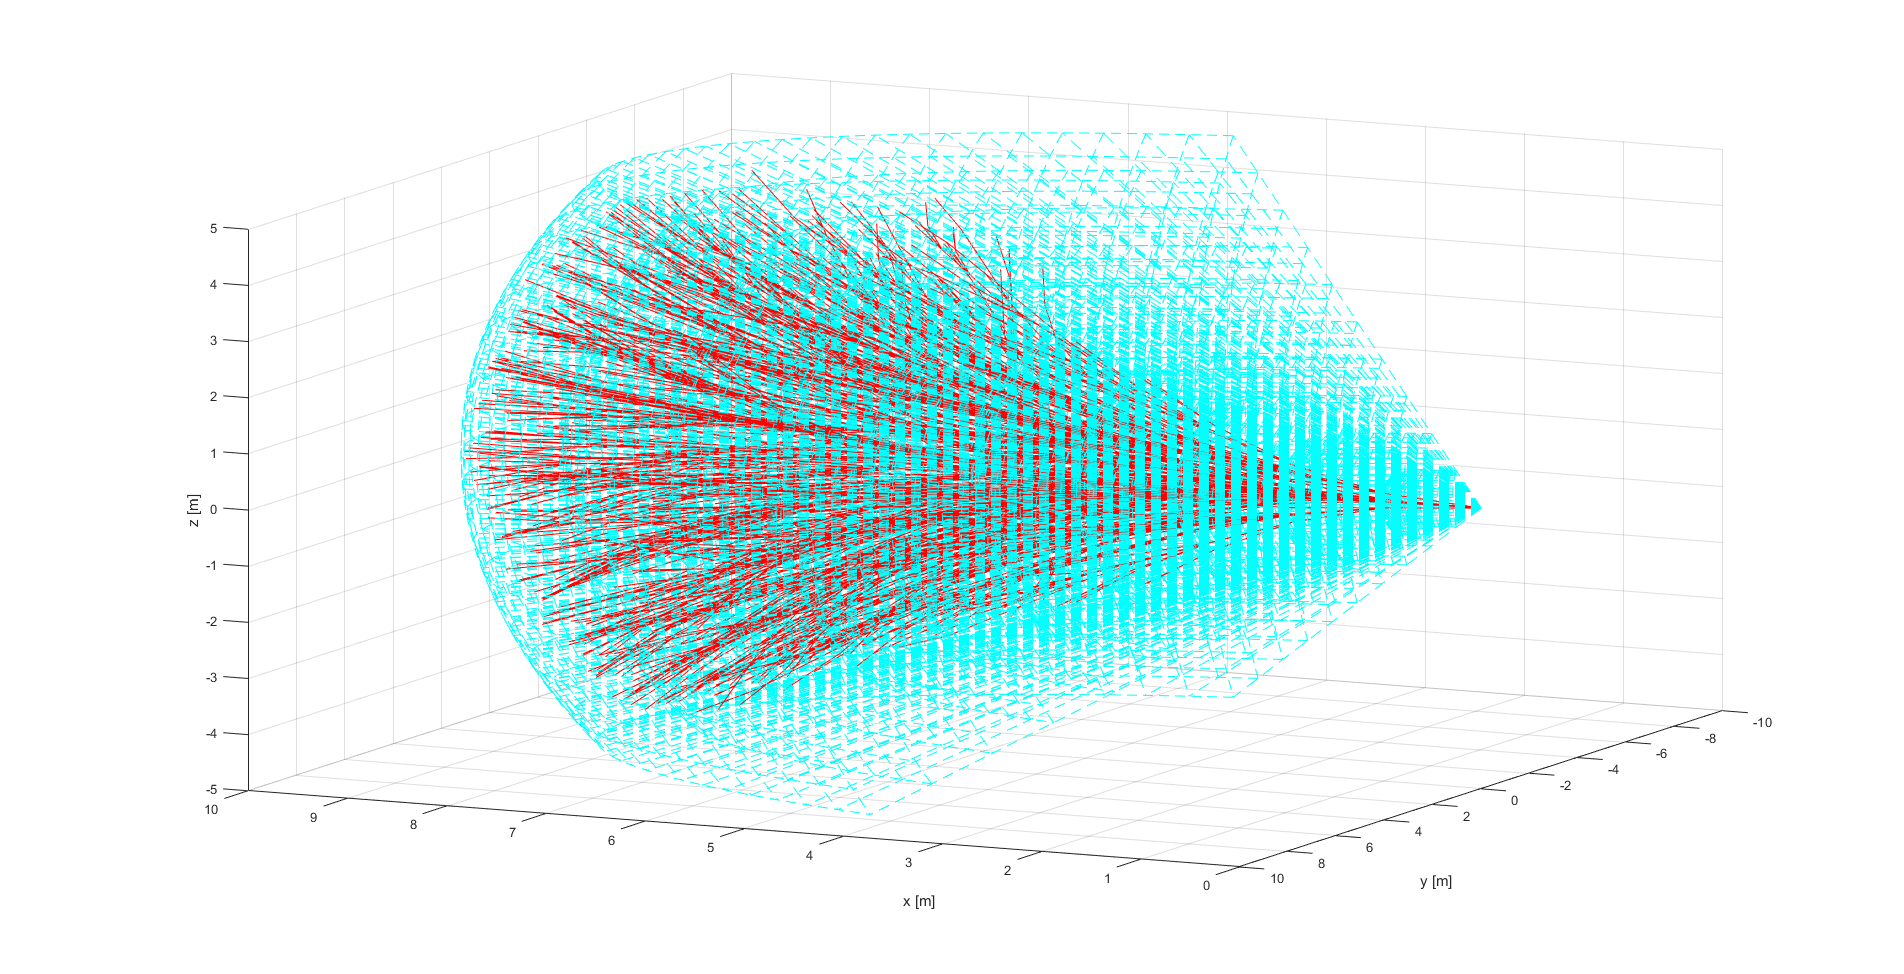
\includegraphics[width=0.95\linewidth]{\FIGDIR/41_Visible_vs_reachable_space.png}
    \caption{Comparison between reachable space and visible space in local coordinates frame.}
    \label{fig:visibleVsReachableLocalFrame}
\end{figure}
\noindent Proposed reach set estimation method have beem used on simplistic plane model from section \ref{sec:3DsimplisticplaneModel} with control strategy $U(t)$ implemented by movement automaton movement set defined in section \ref{sec:3DcontrolSimplisticStrategy}. Final reach set $\mathscr{R}(t_0,t_1,x_0)$ from definition \ref{def:NumericReachSet3D}. is portrayed in visibility grid $\mathscr{G}_{3D}$ in (fig. \ref{fig:visibleVsReachableLocalFrame}).

\subsection{Maximal reach set computation method}\label{s:maxReachSet}
\noindent The first stage of reachable space $\mathscr{R}(t_0,t_1,x_0)$ is computational heavy and its based on prediction of all possible trajectories $\mathscr{T}(x_0,B)$ from def.\ref{def:movementTrajectory}. Each trajectory is defined by movement buffer $B$ from movement automaton $\mathscr{MA}$ movement permutation set $\mathscr{B}(t_1)$ (def. \ref{def:NumericReachSet3D}.). Membership function $\Gamma(c_{i,j,k},\mathscr{T}(x_0,B))$ defined in (def. \ref{def:trajectoryMembershipFunction}.) enables to obtain cell sequence $\mathscr{C}(\mathscr{T}(x_0,B))$ defined in (def. \ref{def:cellSequence}). Cell sequence can be weaved into structure of visibility grid $\mathscr{G}_3D$. Interconnected reach set $\mathscr{R}(t_0,t_1,x_0)$ and visibility grid $\mathscr{G}_{3D}$ for time of scanning $t_i$ results into new structure of \textit{Avoidance grid} $\mathscr{A}(t_i)$. Procedure of avoidance grid creation is described in algorithm \ref{alg:firstStage}.

\begin{algorithm}[H]
    \caption{First stage - calculate maximal reach set.}
    \label{alg:firstStage}
    \SetKwInOut{Input}{Input}
    \SetKwInOut{Output}{Output}
    \Input{Vehicle initial state $x_0$,Vehicle dynamics $\dot{x}=f(x,u)$,\\ Movement Automaton $\mathscr{MA}$, Visibility grid $\mathscr{G}_{3D}$}
    \Output{Avoidance grid $\mathscr{A}(t_i)$}
    $\mathscr{A}(t_i)$=newGrid($t_i,x_0,\dot{x}=f(x,u),\mathscr{MA},\mathscr{G}_{3D}$)\;
    \ForEach{cell $c_{i,j,k}\in\mathscr{A}(t_i)$}{
        $c_{i,j,k}$.status = 'Uncertain'\;
        }
    $t_1\in \R^+$ = maximal escape time \;
    Create movement permutation set $\mathscr{B}(t_i)$\;
    \ForEach{movement buffer $B\in\mathscr{B}(t_i)$}{
        trajectory = $\mathscr{T}(x_0,B)$\;
        cellList = $\mathscr{C}(\mathscr{T}(x_0,B))$\;
        code = hash(cellList)\;
        $\mathscr{A}(t_i)$.trajectoryRegister.put(code,trajectory)\;
        trajectory.cost = trajectory.calculateCost\;
        trajectory.cellSequence=cellList\;
        \ForEach{cell $c_{i,j,k}\in$cellList}{
            state = getState(cell,trajectory)\;
            [entrance,exit] = $\Gamma(c_{i,j,k},\mathscr{T}(x_0,B))$\;
            $c_{i,j,k}$.addTrajectory(code,state,entrance,exit)\;
    }}
\end{algorithm}
\noindent Avoidance grid $\mathscr{A}(t_i)$ for avoidance time $t_i$ represents all possible avoidance trajectories $\mathscr{T}(x_0,B)$ in given visibility grid $\mathscr{G}_{3D}$. Avoidance grid have following properties:
\begin{enumerate}
    \item \textit{Trajectory bounding} - each trajectory $\mathscr{T}(x_0,B)$ in reach set $\mathscr{R}(t_0,t_1,x_0)$ is bounded by positional space occupied by visibility grid $\mathscr{G}_{3D}$.
    \item \textit{Trajectory belonging} - each part of each trajectory $\mathscr{T}(x_0,B)$ in reach set $\mathscr{R}(t_0,t_1,x_0)$ belongs each time of execution to one visibility grid cell $c_{i,j,k}\in\mathscr{G}_{3d}$.
    \item \textit{Trajectory execution-ability} - trajectory $\mathscr{T}(x_0,B)$ with movement buffer $B$ is possible to execute at avoidance time $t_i$ if and only if every cell $c_{i,j,k}$ in trajectory cell sequence is reachable.
    \item \textit{Trajectory cost} - trajectory $\mathscr{T}(x_0,B)$ has given cost of execution for each movement $m_i\in B$ by cost function $J^*(x,u)$.
\end{enumerate}

\subsection{Pruning reach set}
\noindent Second stage of algorithm is much faster than first stage (alg.\ref{alg:firstStage}.), Because it is working with pre-calculated maximal reach set $\mathscr{R}_0(t_0,t_1,x_0)$. To obtain reduced reach set $\mathscr{R}(t_0,t_1,x_0)$ pruning method is introduced in alg. \ref{alg:PruneReachSet}. Visibility grid cells $c_{i,j,k}$ have state which constraints possibilities of vehicle movement. If this status is restrictive, like the cell is \textit{obstacle} or visibility is hindered, therefore cell state is \textit{uncertian}, reach set must be changed to reflect cell status. Trajectory $\mathscr{T}(x_0,B)$ contains movement buffer $B\in\mathscr{MA}$, therefore trajectory can be considered as chain of decisions. Decisions which leads to cells $c_{i,j,k}$ must be removed to maintain reach set $\mathscr{R}$ consistency. Because reach set $\mathscr{R}_0$ is similar to decision tree, application of pruning is feasible \cite{esposito1997comparative}.

\begin{algorithm}[H]
    \caption{Second stage - applying pruning method.}
    \label{alg:PruneReachSet}
    \SetKwInOut{Input}{Input}
    \SetKwInOut{Output}{Output}
    \Input{Target cell for removal $c_{i,j,k}$, Avoidance Grid $\mathscr{A}(t_i)$}
    \Output{Pruned avoidance grid $\mathscr{A}(t_i)$}
    String[] trajectoryCodes = $c_{i,j,k}$.getAllTrajectoryCodes()\;
    \ForEach{code $\in$ trajectoryCodes}{
        trajectory = $\mathscr{A}(t_i)$.getTrajectory(code)\;
        cells = trajectory.cellSequence()\;
        $\mathscr{A}(t_i)$.removeFromRegister(code)\;
        $\mathscr{A}(t_i)$.updateTrajectoryCount()\;
        \ForEach{cell $c_l\in$ cells}{
            $c_l$.removeTrajectory(code)\;
            $c_l$.updateTrajectoryCount()\;
        }
    }
\end{algorithm}
\noindent Because avoidance grid $\mathscr{A}(t_i)$ contains \textit{trajectory register} and each passing trajectory $\mathscr{T}$ is linked to cell $c_i,j,k$ registry. Cross object removal method must be applied. Method to prune reach set $\mathscr{R}$ (alg \ref{alg:PruneReachSet}.)  reflects this fact. Modern object oriented programming languages, like \textit{C++}, enable such implementation \cite{hill1996object}.
	
\subsection{Estimated reach set computation method}\label{ch:estimatedReachSetMethod}
\noindent Let assume that at begin of reach set $\mathscr{R}(t_0,t_1,x_0)$, set of obstacles $\mathscr{O}$ exists. Each obstacle $o\in\mathscr{O}$ is given as point in local coordinate time frame $[d_o,\theta_o,\varphi_o]$, where $d_o$ represents distance, $\theta_o$ represents horizontal angle and $\varphi_o$ represents vertical angle of matter point. Tresholding, filtering and frame shifting are already applied to raw sensor data. Pre-calculated maximal reach set $\mathscr{R}_0(t_0,t_1,x_0)$ is merged to local coordinate frame of avoidance grid $\mathscr{A}(t_i)$. Initial time in reach set is identical to $t_0=t_i$ and final time of reach set $t_1=t_i+t_1$. Initial conditions of system $x_0$ are converted from global coordinate frame to avoidance grid coordinate frame. With well defined offsets, maximal reach set $\mathscr{R}_0$ can be used for any avoidance time $t_i$ and vehicle initial avoidance state $x_i$.

Obstacle avoidance algorithm starts with \textit{initialization of avoidance grid $\mathscr{A}(t_i)$}, where status of each cells $c_{i,j,k}\in\mathscr{A}(t_i)$ status is set as 'Not determined'. For each detected obstacle point in local planar coordinates  $[d_o,\theta_o,\varphi_o]^T$ Obstacle assessment function is given by alg. \ref{alg:06}.
\\
\begin{algorithm}[H]
    \caption{Put obstacle fuction.}
    \label{alg:06}
    \SetKwInOut{Input}{Input}
    \Input{Avoidance grid $\mathscr{A}(t_i)$ grid, Obstacle point $[d_o,\theta_o,\varphi_o]^T$}
    $c_{i,j,k}$=grid.getCell($d_o,\theta_o,\varphi_o$)\;
    \If{$c_{i,j,k}$.status != 'Obstacle'}{
        $c_{i,j,k}$.status = 'Obstacle'\;
        prune($c_{i,j,k}$,${A}(t_i)$)\;
        successors = $c_{i,j,k}$.successors\;
        \ForEach{s $\in$ successors}{
            s.status = 'Uncertain'\;
            prune(s,${A}(t_i)$)\;
        }
    }
\end{algorithm}
\noindent\textit{Obstacle assessment} is done trough application of put obstacle function (alg. \ref{alg:06}.) on each obstacle $o_i$ in detected obstacles set $\mathscr{O}$. At this point every trajectory $\mathscr{T}$ which was passing trough cell with \textit{uncertain} or \textit{obstacle} state is removed. Therefore initial maximal reach set $\mathscr{R}_0(t_0,t_1,x_1)$ is reduced to constrained reach set $\mathscr{R}(t_0,t_1,x_1)$. Avoidance grid $\mathscr{A}(t_i)$ contains cells with \textit{not determined}, \textit{obstacle} and \textit{uncertain} state. Result of alg. \ref{alg:06}. is pruned avoidance grid $\mathscr{A}(t_i)$. Example of pruned avoidance grid $\mathscr{A}(t_i)$ is portrayed in figure \ref{fig:gridObstacleAssessment}. Cells with \textit{obstacle} status are marked as red circles, cells with \textit{uncertain} status are marked as magenta circles and cells with \textit{not determined} status are marked as black stars.
\begin{figure}[H]
    \centering
    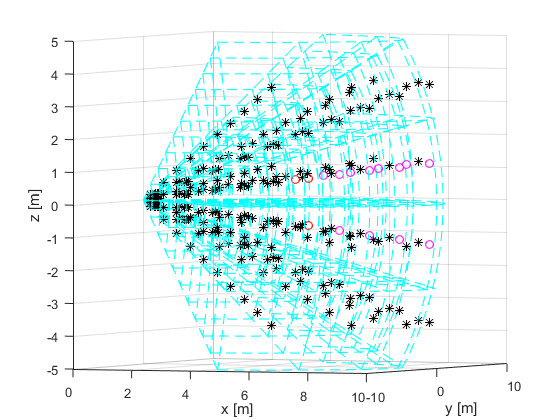
\includegraphics[width=0.6\linewidth]{\FIGDIR/38_Obstacle_assessment_phase.png}
    \caption{Obstacle assessment phase in avoidance grid.}
    \label{fig:gridObstacleAssessment}
\end{figure}

\noindent\textit{Reachability assessment} follows after obtaining pruned avoidance grid $\mathscr{A}(t_i)$. Because pruned avoidance grid $\mathscr{A}(t_i)$ already contains final reach set $\mathscr{R}(t_0,t_1,x_0)$ and hold \textit{trajectory belonging} property, one can say if there exist at least one trajectory $\mathscr{T}(x_0,B)$ to cell $c_{i,j,k}$, cell is reachable. Similar if there does not exist any trajectory $\mathscr{T}(x_0,B)$ to cell $c_{i,j,k}$, cell is unreachable. Reachability/Unreachability assessment is summarized in alg. \ref{alg:reachibilityAssessment}.
\\
\begin{algorithm}[H]
    \caption{Reachibility assessment}
    \label{alg:reachibilityAssessment}
    \SetKwInOut{Input}{Input}
    \SetKwInOut{Output}{Output}
    \Input{Pruned avoidance grid $\mathscr{A}(t_i)$.}
    \Output{Reachable avoidance grid $\mathscr{A}(t_i)$}
    \ForEach{Grid cell $c_{i,j,k}\in \mathscr{A}(t_i)$}{
        \If{$c_{i,j,k}$.status == 'Not determined'}{
            \If{$c_{i,j,k}$.trajectoriesCount()$\ge$ 1}{
                cell.status='Reachable'\;
            }\Else{cell.status='Unreachable'\;}
        }
        
    }
\end{algorithm}
\noindent\textit{Reachability assessment} example is displayed in figure \ref{fig:gridReachabilityAssessment}. Cell status is exact as in figure \ref{fig:gridObstacleAssessment}., cells with \textit{reachable} status are marked as green stars and cells with \textit{unreachable} state are marked as red crosses

\begin{figure}[H]
    \centering
    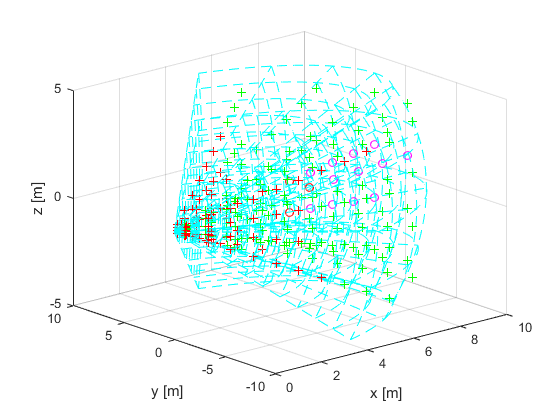
\includegraphics[width=0.6\linewidth]{\FIGDIR/40_Unreachability_assesment_phase.png}
    \caption{Reachibility assessment in avoidance grid.}
    \label{fig:gridReachabilityAssessment}
\end{figure}


\subsection{Avoidance goal selection}\label{ch:avoidanceGoalSimlistic}
\noindent The reachable space $\mathscr{R}$ in avoidance space $\mathscr{A}$ have been estimated. There comes decision where vehicle should fly and which control input should be used to bring vehicle to this point. For theoretical purposes decision making process under uncertainty is omitted. Main purpose of this section is to obtain \textit{avoidance goal} $c_{i,j,k}$ and control input $u(t+t+i)$. Because vehicle is controlled trough movement automaton $\textit{MA}$, movement buffer $B$ will be sufficient for control purposes. Movement automaton $\mathscr{MA}$ can translate movement buffer $B$ to desired control input $u(t+t_i)$.
Let define goal waypoint $\mathscr{WP}$ with global coordinates $[x_g,y_g,z_g]$ and local coordinates $[x_l,\theta_l,\varphi_l]$ in avoidance grid $\mathscr{A}$ coordinate frame. There exist distance function $f(\mathscr{WP},c_{i,j,k})$ which returns euclidean distance between waypoint $\mathscr{WP}$ and center of cell $c_{i,j,k}$. Minimal distance is selection criterion for goal cell $c_{i,j,k}$. Similarly each trajectory $\mathscr{T}(x_0,B)$ belonging to cell $c_{i,j,k}$ have cost $J^*(x,u)$, therefore trajectory movement buffer $B$ for trajectory with minimal cost is selected. Selection process for this simplistic case is summarized in alg. \ref{alg:goalSelectionExample}.  
\begin{algorithm}[H]
    \caption{Example of avoidance goal selection.}
    \label{alg:goalSelectionExample}
    \SetKwInOut{Input}{Input}
    \SetKwInOut{Output}{Output}
    \Input{Avoidance grid $\mathscr{G}_{3D}$, Goal waypoint $\mathscr{WP}_{g}$}
    \Output{Avoidance goal cell $c_{i,j,k}\in\mathscr{A}(t_i)$, Avoidance movement buffer $B$}
    minimalDistance = $\infty$\;
    \ForEach{$c_{i,j,k}\in\mathscr{A}(t_i)$ where $c_{i,j,k}$.status == 'Reachable'}{
        \If{distance($c_{i,j,k},\mathscr{WP}_{g}$) $<$ minimalDistance)}{
            minimalDistance =  distance($c_{i,j,k},\mathscr{WP}_{g}$)\;
            goalCell = $c_{i,j,k}$\;
        }
    }
    minimalCost = $\infty$
    \ForEach{$\mathscr{T}(x_0,B)\in$goalCell}{
        \If{$\mathscr{T}(x_0,B)$.cost $<$ minimalCost}{
            minimalCost =  $\mathscr{T}(x_0,B)$.cost\;
            movementBuffer = $\mathscr{T}(x_0,B)$.buffer\;
        }
    }
    \Return{[goalCell,movementBuffer]}\;
\end{algorithm}

\subsection{Avoidance execution}
\noindent\textit{Avoidance execution} shows reach set estimation method in context of control implementation. Given system $\dot{x}=f(x,u)$ with movement automaton $\mathscr{MA}$ control is controlled via movement buffer $B$, which contains ordered set of movements $\left\{m_1(t_1),\dots,m_j(t_j)\right\}$. Vehicle is equipped with sensor system which have visibility grid $\mathscr{G}_{3D}$. This visibility grid have pre-calculated maximal reach set $\mathscr{R}_0(t_0,t_1,x_0)$ defined by def. \ref{def:NumericReachSet3D}. Visibility grid $\mathscr{G}_{3D}$ and maximal reach set $\mathscr{R}_0(t_0,t_1,x_0)$ are fused into avoidance grid $\mathscr{A}(t_i)$ as defined in section \ref{ch:estimatedReachSetMethod}. Goal for avoidance is determined as described in section \ref{ch:avoidanceGoalSimlistic}. 

Let say vehicle should execute mission plan given by set of waypoints $\left\{\mathscr{WP}_1,\dots,\mathscr{WP}_{n}\right\}$. Movement automaton $\mathscr{MA} $buffer $B$ is flush-able, therefore new ordered set of movements can be inserted after currently processed movement. Avoidance execution is summarized in alg. \ref{alg:avoidanceFramework}. Main cycle is selecting waypoint to reach $\mathscr{WP}$, while inner cycle executes avoidance operation to prevent vehicle collision. Avoidance time $t_i$ is predicted, this time is given as time of last planned movement execution. Empty avoidance grid $\mathscr{A}(t_i)$ for predicted vehicle state $x(t_i)$ is loaded. From visibility grid all augmented obstacles $[d_o,\theta_o,\varphi_o]\in\mathscr{O}$ are put into the avoidance grid (alg. \ref{alg:06}.). Then avoidance goal $c_{i,j,k}$ cell and movement buffer $B$ are selected (alg. \ref{alg:goalSelectionExample}.). Maneuvers obtained from avoidance trajectory $\mathscr{T}(x(t_i),B)$ are inserted into movement automaton $\mathscr{MA}$ execution queue. When vehicle reaches avoidance time $t_i$, movement automaton starts to execute movements $m_j(t_j)\in B$. Defined count of movements is executed in parallel to next avoidance grid $\mathscr{A}(t_{i+1})$ processing. Inner cycle repeats until goal waypoint $\mathscr{WP}_n$ is reached.
\\
\begin{algorithm}[H]
    \label{alg:avoidanceFramework}
    \caption{Obstacle avoidance execution}
    \SetKwInOut{Input}{Input}
    \Input{Mission plan $\left\{\mathscr{WP}_1,\dots,\mathscr{WP}_{n}\right\}$,\\ Plain avoidance grid $\mathscr{A}(t_i),$\\
    Controlled vehicle with $\mathscr{MA}$ control,\\
    Count of executed movements $count$}
    \ForEach{waypoint $\mathscr{WP}_i$ in mission plan}{
    \While{!isWaypointReached($\mathscr{WP}_i$)}{
        $t_i$ = calculateAvoidanceTime($\mathscr{MA}$)\;
        $\mathscr{A}(t_i)$ = loadEmpty$\mathscr{A}(t_i)$()\;
        \ForEach{point $[x_o,\theta_o,\varphi_o]$ in $\mathscr{O}$}{
            putObstacle($\mathscr{A}(t_i)$,$[d_o,\theta_o,\varphi_o]$)(alg. \ref{alg:06}.)\;
            }
        [cell,buffer] = goalSelection($\mathscr{G}_{3D}$,$\mathscr{WP}_i$)(alg. \ref{alg:goalSelectionExample}.)\;
        setMovementBuffer($\mathscr{MA}$,buffer)\;
        executionMovements = getMovements($\mathscr{MA}$,count)\;
        \While{movement $m_j(t_j)\in$executionMovements}{
            $\mathscr{MA}$.executeMovement($m_j$,$t_j$)\;
        }
        }
    }
\end{algorithm}
Proposed avoidance execution with suitable window of opportunity guarantees avoidance of obstacles in environment holding assumptions \ref{ass:1},\ref{ass:3},\ref{ass:4},\ref{ass:5},\ref{ass:6},\ref{ass:7},\ref{ass:8}.